\documentclass{article}
\usepackage{graphicx}
\usepackage{amsmath}
\title{CS181: Final Project Writeup}
\author{Danny Zhu \& Tianhui Cai}

\begin{document}
\maketitle
First we document our observations, then we comment on
a final strategy.

\section{Plant image classification}
We used a neural network to distinguish the plants, implemented using
an adapted version of the code from assignment 2 (included as {\tt
  nn.py}). The input was the 36 binary digits in the image, and the
output was a single real number between 0 and 1.  Based on image data
gathered from data-gathering runs in which a robot visits and eats
every plant within a certain distance of the origin, hence gathering
complete data on the frequencies in that region, we gathered 82591
images of nutritious plants and 272850 images of poisonous plants. We
used 72591 of each for the training data and 1000 each for test and
validation sets. After a little experimentation, it looked like having
a hidden layer didn't help performance, so we went with a simple
two-layer neural network. After a few runs of 20 epochs of training,
we happened to obtain a network with a test performance of $68.3\%$.

We tried various numbers of hidden nodes, but with no discernible
improvement in performance, as demonstrated in figure~\ref{fig:hidden}.

\begin{figure}
  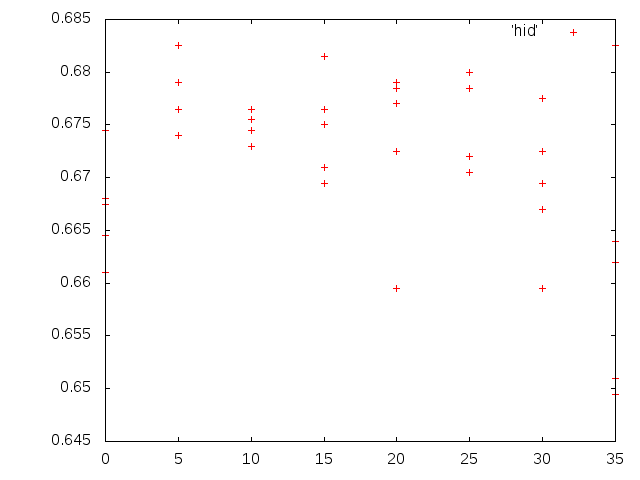
\includegraphics[width=.8\columnwidth]{hid.png}
  \caption{Different numbers of hidden nodes were tested, with five
    trials each.}
  \label{fig:hidden}
\end{figure}

\section{Moving}
\label{sec:moving}
In order to map out the frequency with which nutritious and poisonous
plants appeared in the space, we wrote a strategy ({\tt
  player1.ExploreMoveGenerator}) that moved around the origin in a
spiral pattern, systematically covering all of the spaces near the
origin. By running a few thousand trials, we produced a plot of the
frequency of appearance of nutritious and poisonous plants in each
space. It appears that poisonous plants occur with a constant
frequency of about .15, while nuritious plants have some distribution
peaking at the same value at the origin and decreasing with distance
away from the origin. The distribution appeared approximately
circularly symmetric, so we plotted frequency against distance from
the origin, shown in figure~\ref{fig:plant_freq}. (We made the
assumption that the distribution of nutritious plants is constant
between different games.)

We used Gnuplot to interpolate a function that there is a nutritious
plant at a location of distance $r$ from the origin:
\[\rho(r)=\frac{0.547293}{9.40699+e^{0.553155r-6.93274}}+0.0861578-0.00327286r+3.30966\cdot10^{-5}r^2\]
This function is also graphed in figure~\ref{fig:plant_freq}.

\begin{figure}[h]
  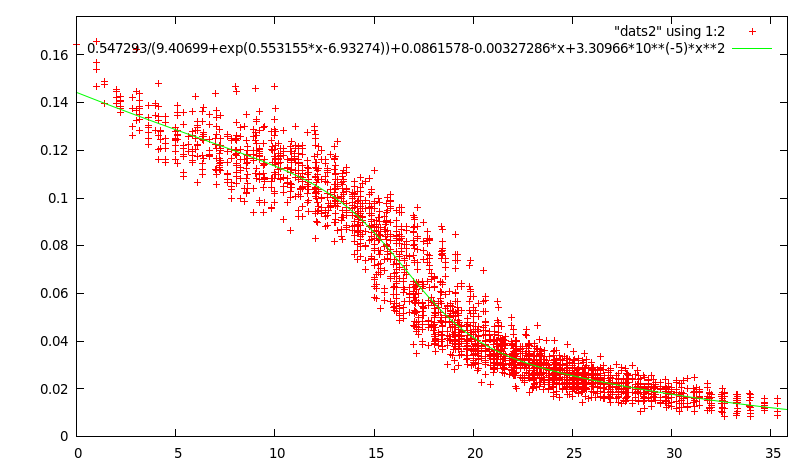
\includegraphics[width=\columnwidth]{nutritiousmodel.png}
  \caption{Density of nutritious plants vs. distance from origin.}
  \label{fig:plant_freq}
\end{figure}

In order to take advantage of the higher concentration of nutritious
plants near the origin, we had the robot move in a spiral around the
origin. To do this, we defined a target square, toward which the robot
tried to move at each step, by the simple strategy of moving toward
the target on the axis (horizontal or vertical) along which the robot
was closer to the target. The target progressed along the spiral each
time the robot reached it.

This had the issue that the robot spent a lot of its time going over
spaces that it had already visited. We tried to think of ways to
reduce this issue, but we decided that it was acceptable, since any
strategy that goes for an exhaustive search of the board will
necessarily spend a lot of its time next to already-seen squares.

\section{Eating by expected reward}
\label{sec:eating}
We should eat if our expected gain is positive. Let $(n,p)$ denote the
number of nutritious and poisonous observations. Let $R_N$ and $R_P$
denote reward/punishment for nutritious or poisonous,
respectively. Let $N,P$ denote the event that the plant is actually
nutritious or poisonous, respectively. Let $c_N$ denote the
probability that our classifier correctly classifies a nutritious
plant, and $c_P$ denote the probability that our classifier correctly
classifies a poisonous plant. We estimated these values using the test
performance of the network, although that neglects variation in rate
of successful classifications between plants. (The appropriateness of
this estimation depends on the image generation model: if it is
independent of position, then it should be okay. But if generation
were done by having a different underlying image for each plant, to
which noise was applied, then that could be violated.)

Finally, $P(N)$ and $P(P)=1-P(N)$ are our priors for a plant being
nutritious or poisonous, given its location, using the formula from
section~\ref{sec:moving}. The expected gain is thus

\begin{align*}
  &R_N P(N|(n,p)) +R_P  P(P|(n,p))\\
  =&\frac{R_NP((n,p)|N) P(N)}{P((n,p)|N)P(N)+P((n,p)|P)P(P)} + \frac{R_PP((n,p)|N)P(N)}{P((n,p)|N)P(N)+P((n,p)|P)P(P)}\\
  =&\frac{R_Nc_N^n(1-c_N)^p P(N)}{ c_N^n(1-c_N)^p P(N) +  c_P^n(1-c_P)^n P(P)} + \frac{R_P c_P^n(1-c_P)^n P(P) }{ c_N^n(1-c_N)^p P(N)+c_P^n(1-c_P)^n P(P)}
\end{align*}

Note that we don't include any ${n+p\choose n}$ term since we have one
sequence of observations, rather than only the number of poisonous and
nutritious observations.  This method is used in the MDP to decide
whether or not to observe which we describe in a later section.

%% \fbox{TODO: DON"T JUST EAT IF IT SAYS NUTRITIOUS. THINK EXPECTED REWARD.}
%% This just seems so un-thought-through. 

\section{Observing}
\subsection{Finite state controller}
We can approach the observing/eating problem instead as a POMDP, and
use a finite state controller to solve both observing and eating.  The
finite state controller hence has $2N+1$ states, with each state
described by $n-p$ where $(n,p)$ is the pair of nutritious and
poisonous observations; we eat if $n-p=N$, reject if $p-n=N$, and
continue observing otherwise.

This appears to work best with $N=1$, i.e. we only look at a first
observation; it appears that with higher $N$, even $N=2$, too many
observations are made. This has the additional shortcoming of not
acting based on expected reward.

%\fbox{TODO:graph of average number observations are made with higher N}\\

%\fbox{TODO: add performance statistics}

\subsection{More sophisticated(?) methods: finite-horizon MDP}
We modeled the problem as a finite-horizon MDP.
\begin{itemize}
\item \emph{States:} $(n,p)$ pairs of observations. As before, we consider
  sequences of observations in which there are $n$ nutritious and $p$
  poisonous observations. 
\item \emph{Actions:} observe or not observe
\item \emph{Rewards:} expected change in energy, given the eating policy
  described in section~\ref{sec:eating}. 
\end{itemize}
This is a finite-horizon MDP because the number of times you would
observe a plant is at most (nutritious plant reward)/(observation cost),
as you would be losing energy with probability 1 if you observed any more
than that. Denote this horizon $H$.
The transition model is predetermined: given $(n,p)$, if we observe,
we can get to either $(n+1,p)$ or $(n,p+1)$; if we don't observe, we
cannot reach any more states. 
The transition probabilities are as follows:
let $N',P'$ denote the events that the next observation is nutritious or poisonous,
respectively; let $N,P$ denote the events that the plant is actually nutritious
or poisonous, respectively; again let $(n,p)$ denote the current observations
and let $P((n,p)|N)$ and $P((n,p)|P)$ be calculated as in section~\ref{sec:eating}.

\[P(N'|(n,p))=P(N'|(n,p),P)P(P|(n,p))+P(N'|(n,p))P(N|(n,p))\]
\[=P(N'|P)P(P|(n,p))+P(N'|N)P(N|(n,p))\]
\[=\frac{P((1,0)|P)P((n,p)|P)P(P)}{P((n,p)|P)P(P)+P((n,p)|N)P(N)} + \frac{P((1,0)|N)P((n,p)|N)P(N)}{P((n,p)|P)P(P)+P((n,p)|N)P(N)}\]

Note that we could have used an HMM with $(n,p)$ as observations 
and nutritious and poisonous to determine these probabilities. 

Hence we solve a dynamic programming problem at every plant we locate,
as the expected rewards and transition probabilities are a function on
the priors, which are location-dependent. This is generally not a time issue,
at least given the default parameters, 
as everything is polynomial in $H$: location is $O(H^3)$ and space is $O(H^2)$. 

%\fbox{TODO: is this equivalent to if we used an HMM? if so, we're in luck.}

\subsection{MDP simplification}
Running the MDP empirically showed that we never request an
observation, and we always eat, until we get far enough from the
center.  This initially seems strange, until you look at $V$ and $Q$
values and realize that the cost per observation is high enough
relative to differences in expected energy gain, and furthermore that
given that reward for eating a nutritious plant is twice the
punishment for eating a poisonous plant, it is almost never the case
even if $(n,p)$ were not always (0,0), that we would decide not to eat
until we had $P(N)$ small enough that the expected change in energy
was negative.

On different parameters, this is not always the case, i.e. if cost of
observation is low enough and if plant reward and plant penalty are
equal, sometimes it will request an observation. But given the default
parameters, this is equivalent to the strategy in which we eat or not
eat using the strategy in section~\ref{sec:eating}, except with
$(n,p)=(0,0)$, i.e.  just use
\[R_NP(N|(n,p))+R_PP(P|(n,p))=R_NP(N)+R_PP(P)\]
where $R_N,R_P$ are reward/punishment for eating nutritious/poisonous
plants and $P(N)$, $P(P)$ are the priors on location from
section~\ref{sec:moving}.

\fbox{TODO: chart performance}

\section{Final Strategy}
We ended up submitting the strategy in which we move as before, but we
decide to eat and observe by just always observing once and eating if
it is nutritious and not eating if it is poisonous. This actually
seems like a terrible idea, especially given that reward for eating a
nutritious plant may be very different (as it is in default
parameters) from the punishment from eating a poisonous plant. It also
totally does not agree with the results from the MDP. But empirically
it appears to be better.

Figure~\ref{fig:comparison} shows a comparison between the strategies
of always eating a plant and eating only when the expected energy gain
is positive.

\begin{figure}
  \begin{center}
    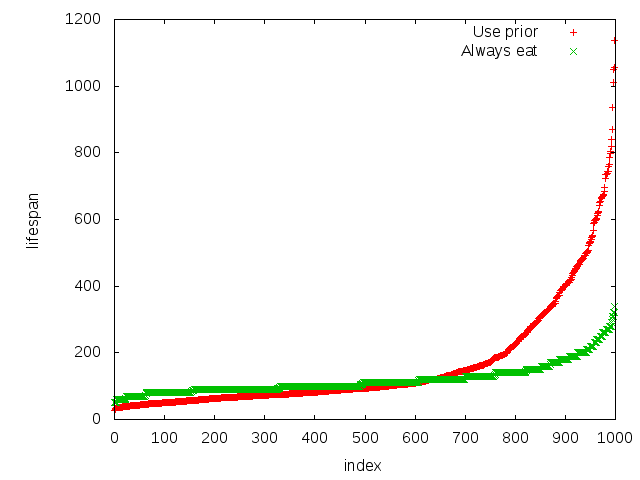
\includegraphics[width=.8\columnwidth]{always_vs_prior.png}
  \end{center}
  \caption{One thousand runs were made using the various strategies,
    the resulting lifespans sorted, and those series plotted together
    here.}
  \label{fig:comparison}
\end{figure}

As you might expect, checking the prior allows the robot to do much
better.

\section{Final remarks}
It is surprising that simple strategies work fairly well, and that it
is often the case that extra information does not end up being useful.

After finding out about how the worlds were generated, we realized
that our biggest shortcoming came from making the assumption that the
distribution of nutritious plants is constant over different runs,
rather than involving three Gaussians randomly placed within a certain
area. Had we not made this assumption, we would have implemented a
moving strategy that was learned on-line rather than off-line.

\end{document}
